\chapter{Selected Gamification Features for English Mind}

Through systematic analysis of existing language learning applications and their gamification implementations, this chapter presents a carefully curated selection of gamification features for English Mind. 

The selection methodology prioritized features that have demonstrated effectiveness in existing applications while maintaining strong alignment with English Mind's core pedagogical principles. Identified features strategically enhance two critical aspects of the learning experience:

\begin{enumerate}
    \item \textbf{Enhanced Practice Experience} 
    \begin{itemize}
        \item Diversified flashcard types
        \begin{itemize}
            \item Word spelling
            \item Word pronunciation
            \item Word-Definition matching
            \item Word-Translation matching
        \end{itemize}
        \item Post-practice review providing immediate feedback and reinforcement
        \item Individual word progress tracking breaking the abstract concept of SRS into tangible stages
    \end{itemize}
    
    \item \textbf{Consistent Practice Motivation} 
    \begin{itemize}
        \item A streak system requiring daily engagement with new vocabulary
    \end{itemize}
\end{enumerate}

\newpage
\section{Diversified Flashcard Types}

The current English Mind's flashcard system employs a single format where users view an English word and recall its meaning. While effective for basic vocabulary acquisition, comparative analysis of language learning applications reveals that the monotony of a single flashcard type can reduce practice effectiveness. The variety in practice formats aims to maintain user interest throughout longer practice sessions, potentially increasing both practice duration and frequency.

This section proposes an expanded word revision system with five distinct flashcard types (see Figure \ref{fig:em-prototype-flashcard-types}), each targeting specific learning objectives.

\begin{enumerate}
    \item \textbf{Recall Meaning}

    The existing English Mind flashcard format, where users see an English word and recall its meaning, will be maintained as the foundation of the practice system. This format effectively tests basic word recognition and meaning recall (see Section \ref{sec:em-active-recall}).

    \item \textbf{Match Words to Translations}
    
    Following successful implementations in applications like Duolingo and WordUp, users match English words with their corresponding translations, presented in sets of five pairs. This format reinforces the connection between words in the target and native languages.

    \item \textbf{Match Words to Definitions}
    
    Similar to the translation matching, this format requires users to match English words with their definitions, reinforcing deeper understanding of word meanings. This format focuses on comprehension rather than translation.

    \item \textbf{Spell Word}
    
    This exercise type presents users with a word's definition and a contextual sentence containing a blank space. Users must correctly spell the target word to complete the sentence. An audio pronunciation button is available as a hint if users cannot determine the required word. The system evaluates spelling accuracy and provides immediate feedback.

    \item \textbf{Pronounce Word}

    Users are shown an English word and prompted to pronounce it correctly. The system evaluates pronunciation accuracy using speech recognition technology, providing binary feedback (correct/incorrect). Understanding that not all practice environments are suitable for speaking exercises, users can opt to skip these cards when needed.

\end{enumerate}
\newpage
\begin{figure}[!h]
    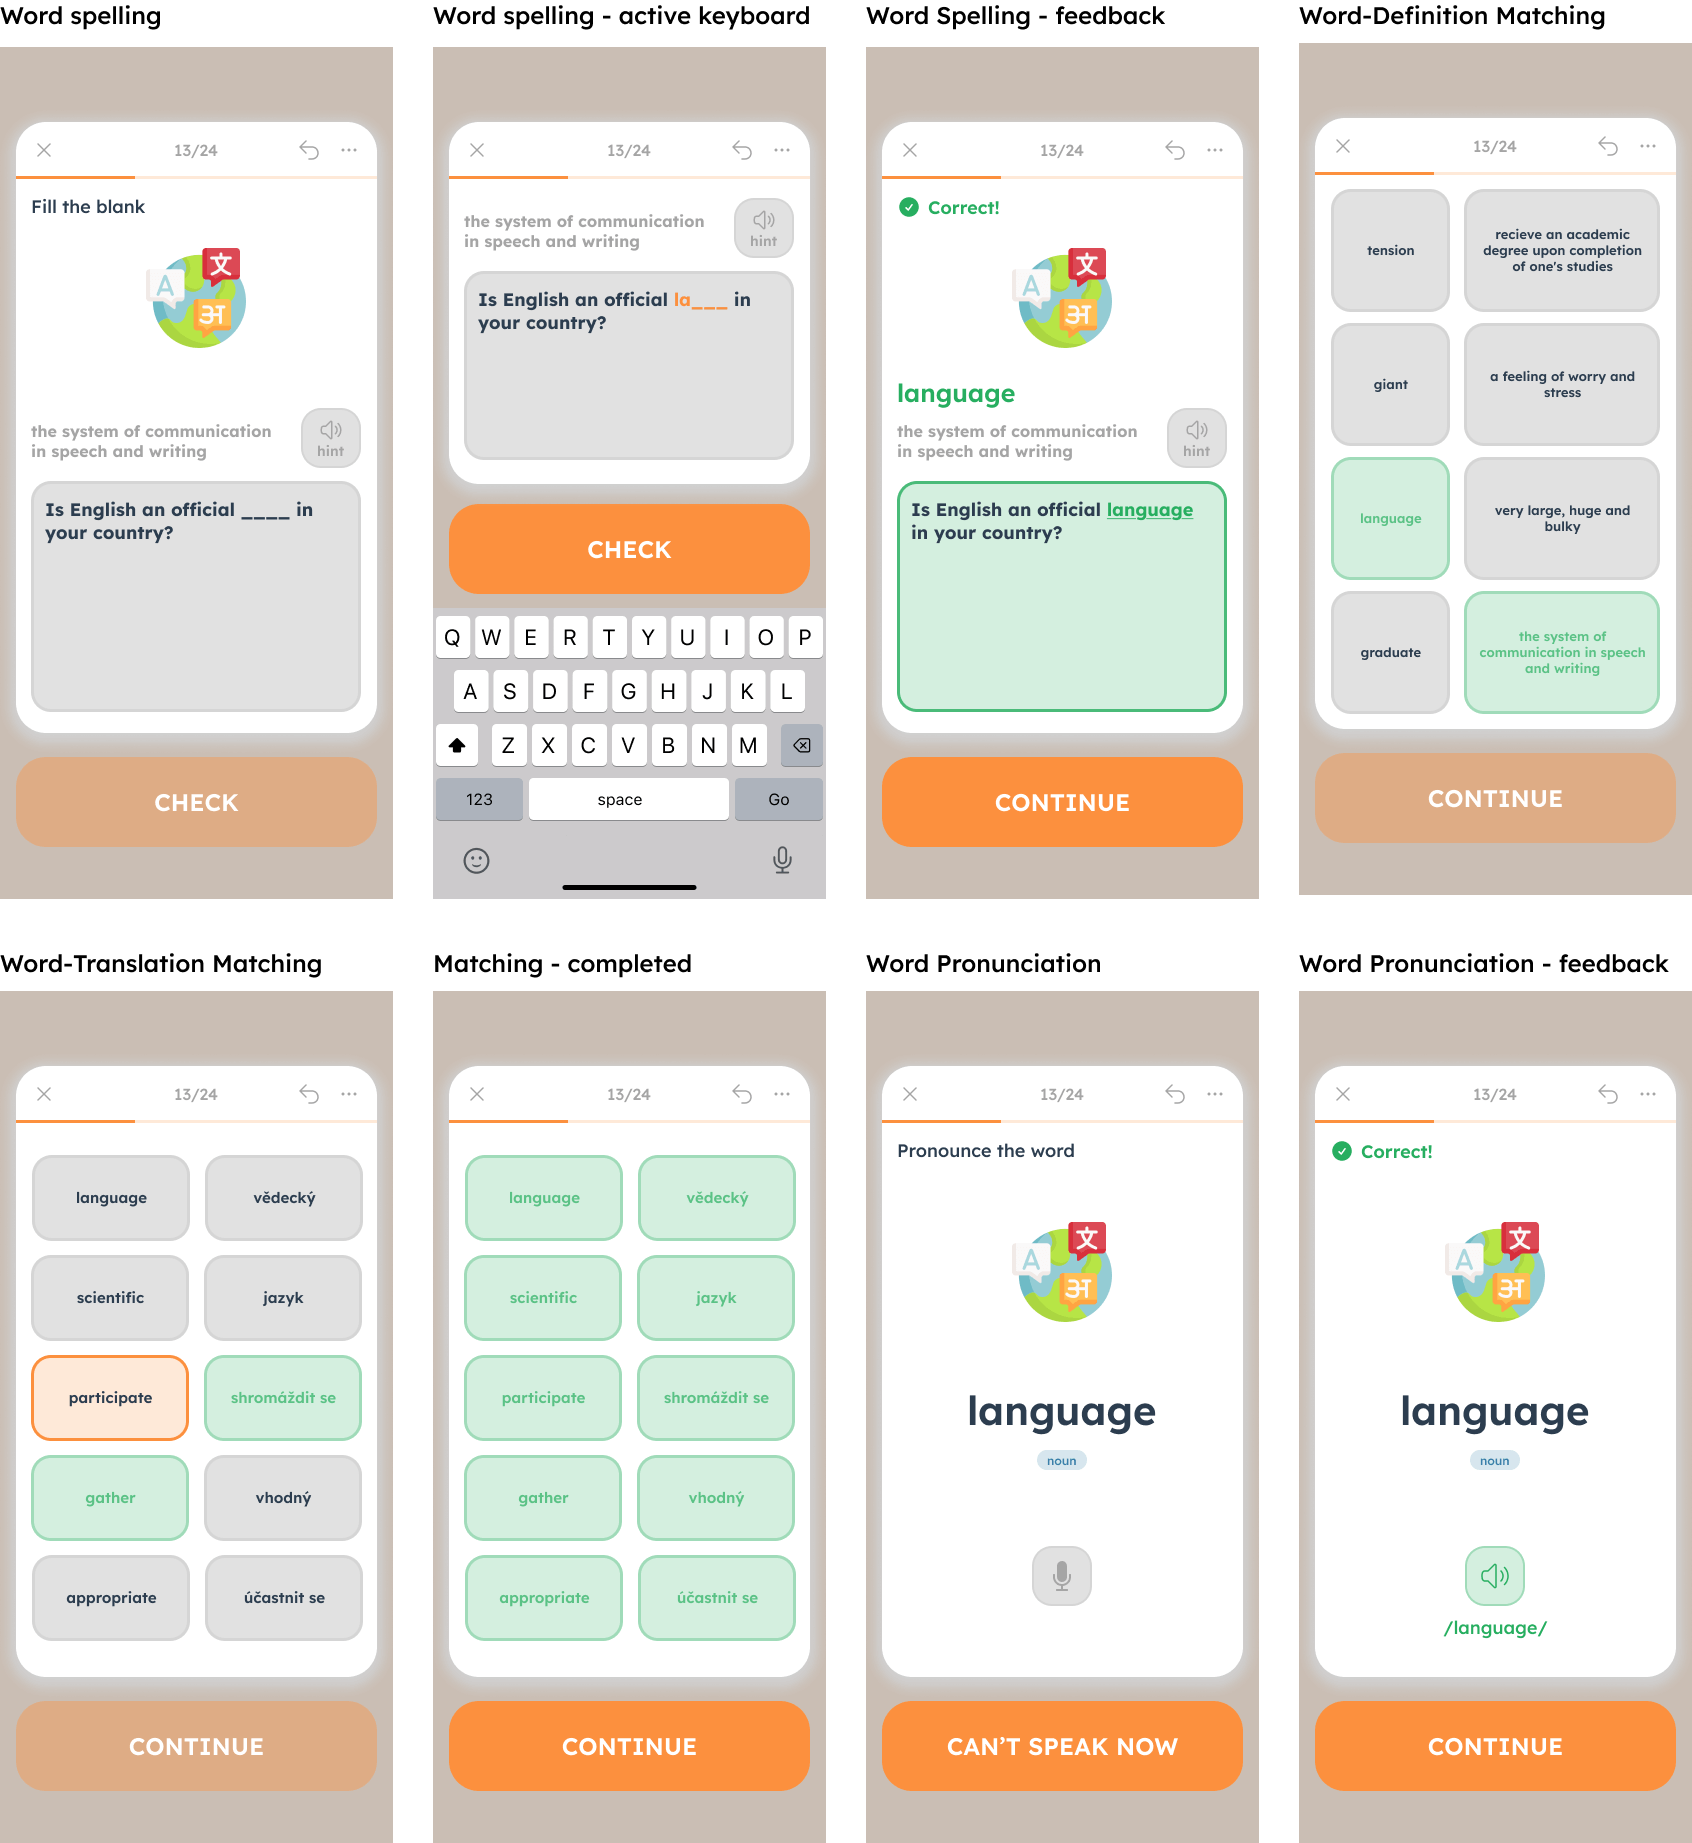
\includegraphics[width=1\textwidth]{src/figures/em-prototype-flashcards.png}
    \caption{Prototype - Flashcard Types}
    \label{fig:em-prototype-flashcard-types}
\end{figure}

The integration of new flashcard types requires careful consideration of the existing spaced repetition system. Only recall meaning flashcards will influence the SRS scheduling of words, while additional types (match, spell, and pronounce) serve as supplementary practice. This approach preserves the proven effectiveness of the current SRS algorithm while enhancing learning through varied practice formats.

The distribution of flashcard types in a practice session follows a structured approach. Recall meaning flashcards appear first and supplementary types follow in randomized order. This prioritization ensures that the core SRS algorithm remains the primary driver of vocabulary acquisition and prevents other flashcard types from inadvertently reminding users of word meanings before they attempt recall.

\section{Vocabulary Progress Tracking}

Inspired by WordUp's individual word progress tracking (see Section \ref{sec:wordup-individual-word-progress-experience}), we propose implementing a visual progress indicator system that integrates seamlessly with English Mind's existing spaced repetition system. This feature provides users with clear, immediate feedback on their progress with each vocabulary item, helping them understand where they stand in the learning journey for specific words. The visual indicator system maps the existing spaced repetition intervals into five distinct stages:
\begin{enumerate}
    \item \textbf{Starting (Stage 1)}
    
    Represents words in their first 3 days after introduction. These words are in the early stages of learning and require frequent review to establish basic recognition.
    
    \item \textbf{Recognizing (Stage 2)}
    
    Covers words in review interval between 1 day and 1 week. During this stage, words still require frequent reviews to build early recall strength and establish memory patterns.
    
    \item \textbf{Reinforcing (Stage 3)}
    
    Includes words with review intervals of 1-3 weeks. At this stage, users can recall words reliably, demonstrating consistent retention with moderate repetition intervals.
    
    \item \textbf{Strengthening (Stage 4)}
    
    Represents words practiced at 3-week to 3-month intervals. Users show strong confidence in recall, requiring significantly less frequent review as the word becomes well-established in long-term memory.
    
    \item \textbf{Mastering (Stage 5)}
    
    Indicates words that have reached intervals of 3-8 months between reviews. These words are approaching full mastery, requiring only rare reviews to maintain retention. Once a word exceeds the 8-month interval, it will be marked as "known" and graduate from the regular review system.
\end{enumerate}

The progress indicator appears only on the recall meaning flashcards (see Figure \ref{fig:em-prototype-word-progress}). It consists of five sequential boxes that fill progressively as the word advances through the stages, providing users with tangible feedback on their learning journey. The visual representation of progress creates a game-like element that enhances motivation and engagement, making the abstract concept of spaced repetition more concrete and understandable.

\begin{figure}[!h]
    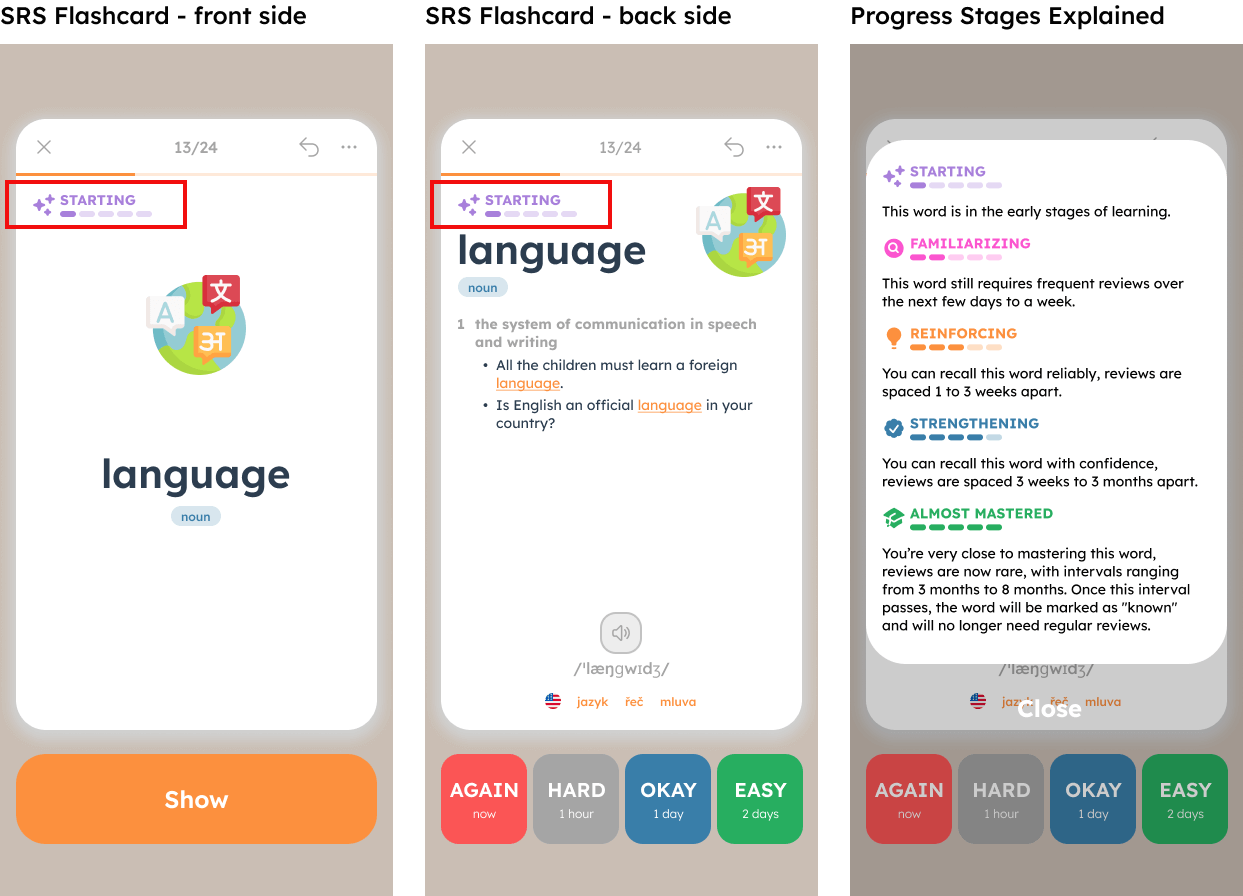
\includegraphics[width=0.95\textwidth]{src/figures/em-prototype-progress-system.png}
    \caption{Prototype: Vocabulary Progress Tracker}
    \label{fig:em-prototype-word-progress}
\end{figure}
\begin{figure}[!h]
    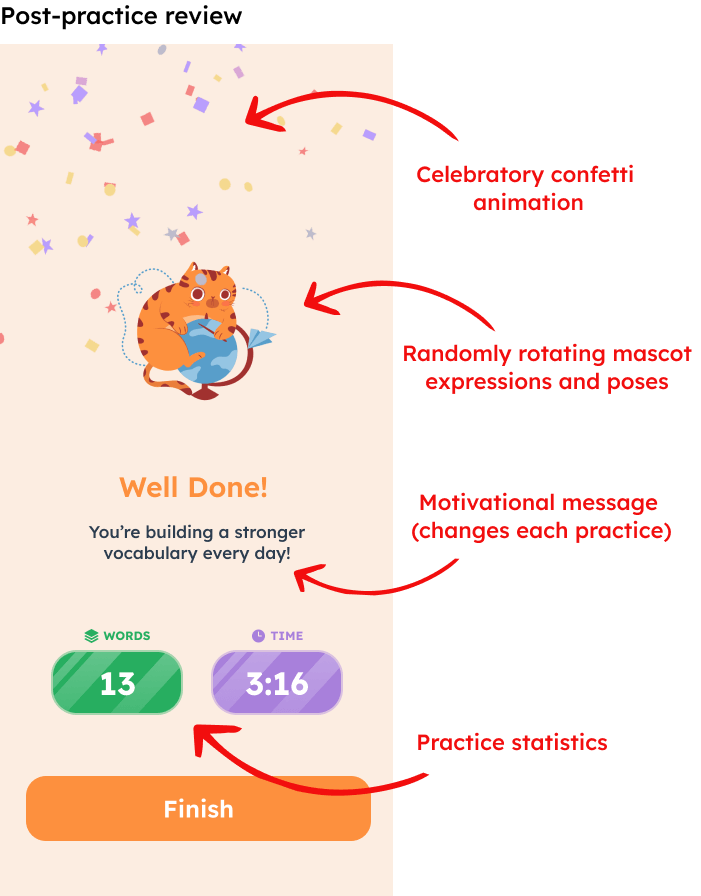
\includegraphics[width=0.55\textwidth]{src/figures/em-prototype-review.png}
    \caption{Prototype: Post-Practice Review}
    \label{fig:em-prototype-practice-review}
\end{figure}

\section{Post-Practice Review}

The post-practice review screen provides immediate feedback after completing a practice session (see Figure \ref{fig:em-prototype-practice-review}). It displays key metrics including the number of words practiced and time spent, accompanied by a brief motivational message. The implementation includes a lightweight confetti animation to provide positive reinforcement for session completion. This feature aims to increase user engagement and potentially increase practice session completion rates.

\section{Streak System}

The streak system is built on the fundamental requirement of learning at least one new word each day to maintain an active streak. Users must mark at least one word as "learning" each day and then review it at their daily queue of flashcards.This requirement ensures meaningful progress while keeping the daily commitment manageable for users. 

To support the effectiveness of the spaced repetition system, new words are strategically placed at the end of the review queue. This placement naturally encourages users to complete their due reviews before accessing the newly added words.

The system intentionally adopts a simplified approach, omitting streak features like "freeze" or streak recovery options. This deliberate choice allows us to establish and validate the core streak mechanics first, while features like streak freezes could be introduced in future iterations based on user feedback and engagement patterns.

\subsection*{Visual Implementation}

The streak counter is prominently displayed at the top of the main screen (see Figure \ref{fig:em-prototype-streak}). This implementation includes a clear numerical display of consecutive practice days, with visual states that reflect the streak's status: a bright, golden appearance for active streaks, and a faded, shadowed appearance when the streak is at risk of being lost.

Upon completing the daily flashcard practice and increasing the streak, a celebration screen appears to reinforce the user's achievement (see Figure \ref{fig:em-prototype-streak}). This screen showcases the updated streak count alongside a weekly progress view displaying the current week's streak activity (Monday through Sunday). When users maintain a perfect week of daily practice, these seven days are highlighted within a special golden frame, providing additional visual recognition for consistent engagement.

\begin{figure}[!h]
    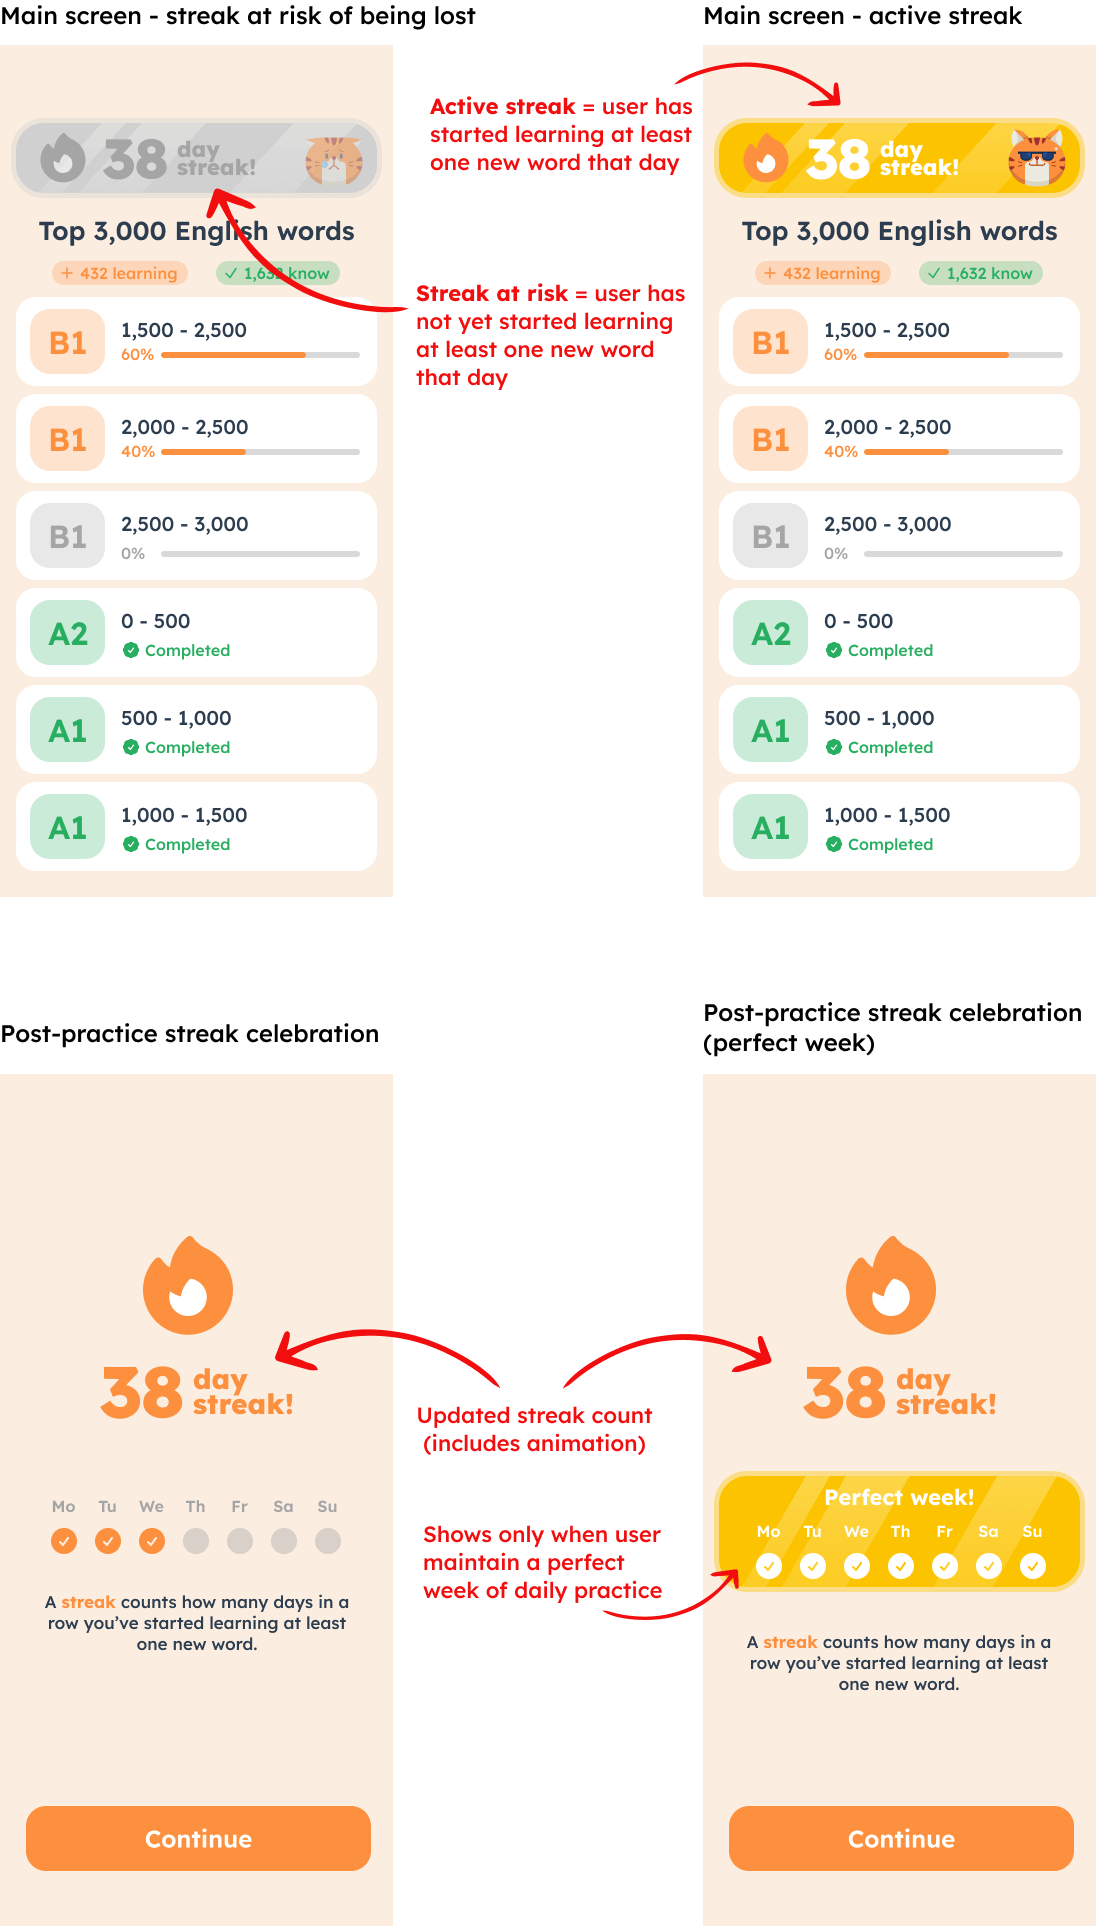
\includegraphics[width=0.9\textwidth]{src/figures/em-prototype-streak.png}
    \caption{English Mind - Prototype: Streak Implementation}
    \label{fig:em-prototype-streak}
\end{figure}

\subsection*{Expected Impact}

The streak system is designed to serve multiple pedagogical and motivational purposes:

\begin{itemize}
    \item \textbf{Establish Daily Practice Habits:} By providing a clear, visible metric for consistency, it helps users establish and maintain daily practice habits.
    
    \item \textbf{Encourage Complete Reviews:} The strategic placement of new words after due flashcards naturally encourages users to complete their spaced repetition queue.
\end{itemize}
